\documentclass[11pt]{charter}

% El títulos de la memoria, se usa en la carátula y se puede usar el cualquier lugar del documento con el comando \ttitle
\titulo{Desarrollo de un sistema embebido para un titulador potenciométrico automático} 

% Nombre del posgrado, se usa en la carátula y se puede usar el cualquier lugar del documento con el comando \degreename
\posgrado{Carrera de Especialización en Sistemas Embebidos} 
%\posgrado{Carrera de Especialización en Internet de las Cosas} 
%\posgrado{Carrera de Especialización en Intelegencia Artificial}
%\posgrado{Maestría en Sistemas Embebidos} 
%\posgrado{Maestría en Internet de las cosas}

% Tu nombre, se puede usar el cualquier lugar del documento con el comando \authorname
\autor{Fernando Ezequiel Daniele} 

% El nombre del director y co-director, se puede usar el cualquier lugar del documento con el comando \supname y \cosupname y \pertesupname y \pertecosupname
\director{Javier Andrés Redolfi}
\pertenenciaDirector{UTN FRSFCO} 
% FIXME:NO IMPLEMENTADO EL CODIRECTOR ni su pertenencia
\codirector{} % si queda vacio no se deberíá incluir 
\pertenenciaCoDirector{}

% Nombre del cliente, quien va a aprobar los resultados del proyecto, se puede usar con el comando \clientename y \empclientename
\cliente{María Eugenia Taverna}
\empresaCliente{GISAI - UTN FRSFCO}

% Nombre y pertenencia de los jurados, se pueden usar el cualquier lugar del documento con el comando \jurunoname, \jurdosname y \jurtresname y \perteunoname, \pertedosname y \pertetresname.
\juradoUno{Nombre y Apellido (1)}
\pertenenciaJurUno{pertenencia (1)} 
\juradoDos{Nombre y Apellido (2)}
\pertenenciaJurDos{pertenencia (2)}
\juradoTres{Nombre y Apellido (3)}
\pertenenciaJurTres{pertenencia (3)}
 
\fechaINICIO{22 de junio de 2020}		%Fecha de inicio de la cursada de GdP \fechaInicioName
\fechaFINALPlanificacion{22 de Agosto de 2020} 	%Fecha de final de cursada de GdP
\fechaFINALTrabajo{31 de junio de 2021}		%Fecha de defensa pública del trabajo final

\usepackage[section]{placeins}

\begin{document}

\maketitle
\thispagestyle{empty}
\pagebreak


\thispagestyle{empty}
{\setlength{\parskip}{0pt}
\tableofcontents{}
}
\pagebreak


\section{Registros de cambios}
\label{sec:registro}


\begin{table}[ht]
\label{tab:registro}
\centering

\begin{tabularx}{\linewidth}{@{}|c|X|c|@{}}
\hline
\rowcolor[HTML]{C0C0C0} 
\hline
Revisión & \multicolumn{1}{c|}{\cellcolor[HTML]{C0C0C0}Detalles de los cambios realizados} & Fecha      \\ \hline
1.0      & Creación del documento                                                          & 22/06/2020 \\ \hline
1.1      & Entrega semanas 2 - 3                                         & 11/07/2020 \\ 
\hline
1.2      & Correciones entrega semanas 2 - 3 & 18/07/2020  \\
\hline
1.3      & Entrega semanas 3 - 4 & 31/07/2020  \\ \hline
1.4      & Se cambiaron requerimentos & 05/08/2020 \\ \hline
1.5      & Entrega semanas 4 - 5 & 07/08/2020  \\ \hline
%		   Con texto partido \newline
%		   En varias líneas \newline
%		   A propósito                                                                     & dd/mm/aaaa \\ \hline
\end{tabularx}
\end{table}

\pagebreak



\section{Acta de constitución del proyecto}
\label{sec:acta}

\begin{flushright}
Buenos Aires, \fechaInicioName
\end{flushright}

\vspace{2cm}

Por medio de la presente se acuerda con el Ing. \authorname\hspace{1px} que su Trabajo Final de la \degreename\hspace{1px} se titulará ``\ttitle'', consistirá esencialmente en el prototipo preliminar de un sistema para el control de un titulador o valorador, y tendrá un presupuesto preliminar estimado de 640 hs de trabajo y \$15.000, con fecha de inicio \fechaInicioName\hspace{1px} y fecha de presentación pública \fechaFinalName.

Se adjunta a esta acta la planificación inicial.

\vfill

% Esta parte se construye sola con la información que hayan cargado en el preámbulo del documento y no debe modificarla
\begin{table}[ht]
\centering
\begin{tabular}{ccc}
\begin{tabular}[c]{@{}c@{}}Ariel Lutenberg \\ Director posgrado FIUBA\end{tabular} &  & \begin{tabular}[c]{@{}c@{}}\clientename \\ \empclientename \end{tabular} \vspace{2.5cm} \\ 
\multicolumn{3}{c}{\begin{tabular}[c]{@{}c@{}} \supname \\ Director del Trabajo Final\end{tabular}} \vspace{2.5cm} \\
\begin{tabular}[c]{@{}c@{}}\jurunoname \\ Jurado del Trabajo Final\end{tabular}     &  & \begin{tabular}[c]{@{}c@{}}\jurdosname\\ Jurado del Trabajo Final\end{tabular}  \vspace{2.5cm}  \\
\multicolumn{3}{c}{\begin{tabular}[c]{@{}c@{}} \jurtresname\\ Jurado del Trabajo Final\end{tabular}} \vspace{.5cm}                                                                     
\end{tabular}
\end{table}




\section{Descripción técnica-conceptual del proyecto a realizar}
\label{sec:descripcion}

El prototipo en particular que se desarrollará forma parte de un proyecto interdisplinar gestado en el Grupo de Investigación Sobre Aplicaciones Inteligentes (GISAI) de la Universidad Tecnológica Nacional Facultad Regional San Francisco (UTN FRSFCO), cuyo objetivo es el desarrollo de un titulador potenciométrico automático para el laboratorio de servicios de la facultad. El proyecto involucra docentes y alumnos de cuatro carreras de ingeniería, cuyas actividades se detallan a continuación:
\begin{itemize}
	\item Ingeniería química: aporta el conocimiento sobre el proceso de titulación y establece los requerimentos que deberá tener el sistema. 
	\item Ingeniería electromecánica: se encarga de diseñar y construir una bomba peristátilca y las partes mecánicas. 
	\item Ingeniería en sistemas de información: se encarga de desarrollar un software para el procesamiento de los datos del cliente y los datos obtenidos del titulador. 
	\item Ingeniería electrónica: se encarga de diseñar el sistema embebido para el control automático del titulador. 
\end{itemize}
El proyecto surge de la iniciativa del grupo GISAI de encarar un proyecto que involucre las cuatro ingenierías que forman parte de la UTN FRSFCO. Es en esa iniciativa que se propone el desarrollo de un titulador potenciométrico automático.\\
Las titulaciones, también conocidas como valoraciones, son ampliamente utilizadas en química analítica para determinar la concentración de ácidos, bases, agentes oxidantes, agentes reductores, iones metálicos, proteínas y muchas otras especies químicas. Son métodos poderosos de análisis que se basan en la reacción de estequiometría definida, que se da entre un analito y un reactivo estándar conocido como titulante o valorante.\\
Las titulaciones pueden ser realizadas en forma manual o automática. Actualmente existen en el mercado tituladores de operación automatizada que determinan la concentración de diferentes analitos, pero estos equipos son económicamente inaccesibles para universidades y laboratorios en los que existe una frecuencia baja de muestras a analizar. Estas dificultades traen aparejada poca celeridad en la obtención de resultados de manera convencional y vuelve a los laboratorios universitarios poco competentes frente a la demanda de análisis.\\
 La UTN FRSFCO no cuenta con equipos automatizados para la realización de distintos ensayos útiles en las áreas de ingeniería química y electromecánica. El por eso que el proyecto general busca desarrollar un prototipo de titulador automático para el empleo en diferentes valoraciones ácido-base.\\
 Este prototipo se destinará a la automatización de los procesos de titulación manuales llevados a cabo en el laboratorio de servicios a terceros que funciona en la universidad, así como también en los grupos de I+D, y cátedras de la carrera de ingeniería química y electromecánica, que utilizan este tipo de técnicas.\\
El caso de este proyecto en particular se enfoca en el desarrollo del sistema embebido que será el encargado de automatizar el proceso de titulación. Este proceso consiste en inyectar mediante la bomba la solución titulante en la muestra a analizar. Durante todo el proceso se debe realizar la lectura del potencial que entrega un electrodo de pH situado en el recipiente de la muestra, y tabular los datos del potencial y de volumen añadido para poder obtener la curva de titulación. A través de estos datos es posible determinar el volumen (o los volúmenes) de titulante correspondiente al momento en el cual la curva posee un punto de inflexión, es decir, cuando la derivada segunda del potencial respecto al volumen utilizado de titulante se hace cero. Ese valor es el que utilizará el software y el analista para determinar la sustancia desconocida.\\
El presente proyecto se destaca especialmente porque sienta las bases de un trabajo interdisciplinar, enfocado en obtener un producto económico, de código y hardware abierto, adecuado a las necesidades de la facultad, y con la posibilidad de realizar modificaciones o mejoras futuras.\\
En la Figura \ref{fig:diagBloques} se presenta el diagrama en bloques del sistema. A continuación se detallan cada uno de sus componentes:
\begin{itemize}
\item Módulo ESP32-DevKitC: incluye un microprocesador dual Core de 32 bits y WiFi integrado, entre otros. El microprocesador es el encargado de controlar el resto de los componentes. En cuanto al WiFi, será el medio de conexión para que un usuario pueda acceder a una página web almecenada en la memoria del módulo, y visualizar los datos obtenidos en el proceso de titulación.
\item Interfaz de usuario: compuesta por una pantalla TFT táctil de 2,4 pulgadas. Le permitirá al usuario configurar el dispositivo, realizar la calibración del mismo, dar inicio al proceso de titulación y visualizar datos.
\item Lector de tarjetas SD: se encuentra en el mismo módulo de la pantalla, donde se guardarán los datos obtenidos en la titulación.
\item Bomba peristáltica: se encarga de dosificar el titulante en el recipiente de la muestra.
\item Electrodo: es el encargado de realizar la medición de pH.
\item Agitador: compuesto por un motor de CC. Realiza la mezcla el titulante con la muestra.
\item Sensor de temperatura: puede o no situarse en el recipiente de la muestra.
\end{itemize}


%\vspace{25px}



%\vspace{25px}



\section{Identificación y análisis de los interesados}
\label{sec:interesados}

%Nota: (borrar esto y todas las consignas en color rojo antes de entregar este documento).
 
%Es inusual que una misma persona esté en más de un rol, incluso en proyectos chicos.
 
%Si se considera que una persona cumple dos o más roles, entonces sólo dejarla en el rol más importante. Por ejemplo:

%\begin{itemize}
%\item Si una persona es Cliente pero también colabora u orienta, dejarla solo como Cliente.
%\item Si una persona es el Responsable, no debe ser colocado también como Miembro del equipo.
%\end{itemize}

%Pero en cambio sí es usual que el Cliente y el Auspiciante sean el mismo, por ejemplo.

\begin{table}[ht]
%\caption{Identificación de los interesados}
%\label{tab:interesados}
\begin{tabularx}{\linewidth}{@{}|l|X|X|l|@{}}
\hline
\rowcolor[HTML]{C0C0C0} 
Rol           & Nombre y Apellido & Organización 	& Puesto 	\\ \hline
Cliente       & \clientename      &\empclientename	& Co-Directora de proyecto    	\\ \hline
%Impulsor      &        -          &      -        	&    -    	\\ \hline
Responsable   & \authorname       & FIUBA        	& Alumno 	\\ \hline
Colaborador & Leonardo Anchino  & GISAI - UTN    	& Becario      	\\ \hline
Colaborador & Lorenzo Depetris  & GISAI - UTN    	& Becario      	\\ \hline
Orientador    & \supname	      & \pertesupname 	& Director	Trabajo final \\ \hline
%Equipo        & % miembro1 \newline 
%						 -         &   -           	&  -      	\\ \hline
%Opositores    &      -            &   -           	&  -      	\\ \hline
Usuario final & Laboratorio de Servicios & UTN FRSCO & -        	\\ \hline
\end{tabularx}
\end{table}

%El Director suele ser uno de los Orientadores.
%No dejar celdas vacías; si no hay nada que poner en una celda colocar un signo ``-''.
%No dejar filas vacías; si no hay nada que poner en una fila entonces eliminarla.
%Sería deseable listar a continuación de la tabla las principales características de cada interesado.
 
%Por ejemplo:
%\begin{itemize}
%\item Auspiciante: es riguroso y exigente con la rendición de gastos. Tener mucho cuidado con esto.
%\item Equipo: Juan Perez, suele pedir licencia porque tiene un familiar con una enfermedad. Planificar considerando esto.
%\item Orientador: María Gómez, nos va a poder ayudar mucho con la gestión de impuestos.
%\end{itemize}

\begin{figure}[htpb]
\centering 
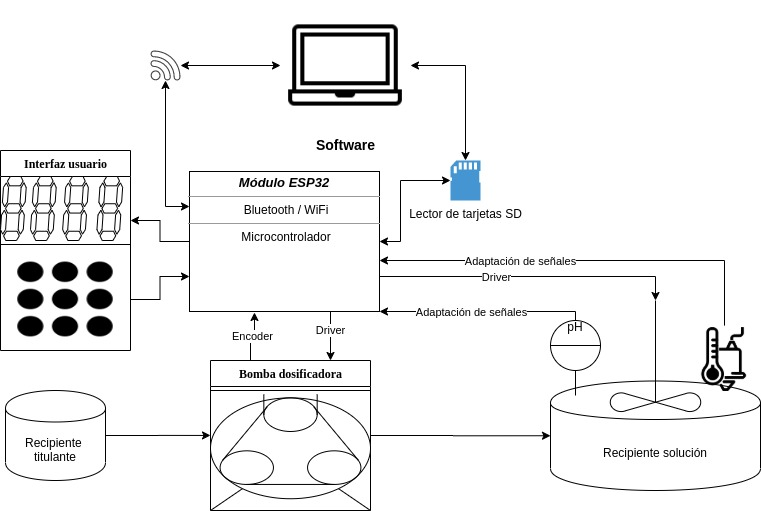
\includegraphics[width=1\textwidth]{./Figuras/diagBloques.jpg}
\caption{Diagrama en bloques del sistema}
\label{fig:diagBloques}
\end{figure}

\section{1. Propósito del proyecto}
\label{sec:proposito}


El propósito de este proyecto es desarrollar el prototipo de un sistema embebido que permita automatizar y controlar el ensayo de titulación potenciométrica.


\section{2. Alcance del proyecto}
\label{sec:alcance}

El proyecto incluye:
\begin{itemize}
\item Una interfaz de usuario que permite la configuración y calibración del dispositivo, asi como también dar inicio al proceso de titulación.
\item La visualización de la curva de potencial respecto al volumen de titulante inyectado.
\item El control de la bomba que inyecta el titulante en la muestra
\item El cálculo y visualización del resultado de la titulación. El resultado es el volumen de titulante utilizado al momento de producirse un punto de inflexión en la curva.
\item El almacenamiento de los datos del ensayo en una memoria SD
\item La visualización de los datos del ensayo en una página web, a través de una conexión wifi local.
\end{itemize}

\vspace{25px}

El proyecto no incluye:
\begin{itemize}
\item El manejo del dispositivo de manera remota.
\item El diseño de gabinetes u otras partes mecánicas. 
\end{itemize}

\section{3. Supuestos del proyecto}
\label{sec:supuestos}

Para el desarrollo del presente proyecto se supone que:

\begin{itemize}
\item El desarrollo de la bomba peristáltica y demás partes mécanicas estarán desarrolladas en el tiempo previsto.
\item El dinero disponible será suficiente para la adquisición de los materiales en el contexto macroeconómico actual
\item El aislamiento y/o distanciamento preventivo social y obligatorio no impidedirá la adquisición de materiales ni retrasará las pruebas y verificaciones del dispositivo.
\end{itemize}

\section{4. Requerimientos} %Los requerimientos deben numerarse y de ser posible agruparlos por afinidad:
\label{sec:requerimientos}

\begin{enumerate}
\item Interfaces Externas
	\begin{enumerate}
	\item El hardware deberá contar con una pantalla TFT táctil. [TPA-ERH-01-REQ001]
	\item El hardware deberá contar con un lector de tarjetas SD. [TPA-ERH-01-REQ002]
	\item El hardware deberá contar con un driver para un motor paso a paso Nema 17. [TPA-ERH-01-REQ003]
	\item El hardware deberá contar con una entrada para un electrodo de pH. [TPA-ERH-01-REQ004]
\end{enumerate}
	
\item Funciones
	\begin{enumerate}
	\item El usuario podrá elegir mediante la pantalla táctil los valores de tres muestras patrones (buffers) que se utilizarán en la calibración. [TPA-ERS-01-REQ001]
El usuario podrá elegir mediante la pantalla táctil el volumen de corte de la titulación. [TPA-ERS-01-REQ002]
	\item El usuario podrá elegir mediante la pantalla táctil si utilizar o no el agitador. Cuando el proceso de titulación comience, el agitador debe activarse si así lo indicó el usuario. [TPA-ERS-01-REQ003]
	\item El usuario podrá realizar mediante la pantalla táctil el proceso de calibración con cada uno de los tres buffers. [TPA-ERS-01-REQ004]
	\item Los valores de potencial obtenidos en el proceso de la calibración se deben guardar en la memoria flash del ESP32. [TPA-ERS-01-REQ005]
	\item El valor de pH se debe calcular de manera proporcional a la recta de ajuste de los valores de potencial obtenidos en la calibración. [TPA-ERS-01-REQ006]
	\item El usuario podrá dar inicio al proceso de titulación mediante la pantalla táctil. [TPA-ERS-01-REQ007]
	\item Durante la titulación, la pantalla debe mostrar el valor actual leído en mV y en pH y una gráfica de pH en el eje de la ordenadas y de volumen de titulante añadido en el eje de las abcisas. [TPA-ERS-01-REQ008]
	\item Cada valor de volumen añadido junto al valor de potencial asociado durante el proceso de titulación deben almacenarse en un archivo de texto en la tarjeta sd. No es necesario que esto se haga en tiempo real. Al iniciar otro proceso de titulación, los datos de la titulación anterior serán eliminados. [TPA-ERS-01-REQ009]
	\item Cada valor de volumen añadido junto al valor de potencial asociado durante el proceso de titulación deben mostrarse en una página web almacenada en la memoria flash. [TPA-ERS-01-REQ010]
	\item El usuario podrá acceder a la página web mediante una conexión wifi. No es necesario que esto se haga en tiempo real. [TPA-ERS-01-REQ011]
	\item El sistema deberá ser capaz de leer y mostrar el potencial entregado por un electrodo de pH, con una resolución de 1 mV para la lectura del potencial y de 0.01 pH para su conversión a pH. Para ello se utilizará el conversor analógico de 12 bits incorporado en el ESP32. [TPA-ERS-01-REQ012]
	\item El sistema deberá enviar pulsos de 10 ms de ciclo útil al pin step del módulo dvr8825. El tiempo mínimo de espera entre cada pulso debe ser de 1 segundo luego que la lectura de potencial se haya estabilizado. El sistema dejará de enviar los pulsos cuando se haya inyectado la cantidad de volumen indicada por el usuario como volumen de corte. [TPA-ERS-01-REQ013]
	\item Cada pulso se corresponde con el incremento de TBD mL en la cantidad de volumen inyectado, comenzando por un nivel de 0 mL. [TPA-ERS-01-REQ014]

\end{enumerate}

\item Requisitos de Rendimiento
	\begin{enumerate}
	\item El sistema deberá ser capaz de realizar titulaciones que involucren una cantidad mínima de 50 ml 	\item de titulante y una cantidad máxima de 100 ml. [TPA-ERS-01-REQ015]
	\end{enumerate}
	
\item Restricciones de Diseño
	\begin{enumerate}
	\item Se utilizará el módulo ESP32 como computadora principal. [TPA-ERS-01-REQ016]
	\end{enumerate}
	
\item Requisitos Futuros
	\begin{enumerate}
	\item El dispositivo contará con un control de lazo cerrado para la medición de volumen y el control de la bomba.
	\item El usuario podrá acceder a todas la funcionalidades de manera remota mediante conexión WiFi o Bluetooth.
	\end{enumerate}
\end{enumerate}


\section{Historias de usuarios (\textit{Product backlog})}
\label{sec:backlog}

\begin{consigna}{red}
Descripción: En esta sección se deben incluir las historias de usuarios y su ponderación (\textit{history points}). Recordar que las historias de usuarios son descripciones cortas y simples de una característica contada desde la perspectiva de la persona que desea la nueva capacidad, generalmente un usuario o cliente del sistema.

La ponderación es un número entero que representa el tamaño de la historia comparada con otras historias de similar tipo.
\end{consigna}


\section{5. Entregables principales del proyecto}
\label{sec:entregables}

\begin{itemize}
\item Prototipo funcional
\item Manual de uso
\item Diagrama esquemático
\item Código fuente
\item Memoria técnica
\end{itemize}

\section{6. Desglose del trabajo en tareas}
\label{sec:wbs}

\begin{enumerate}
\item Investigación y documentación (60 hs)
	\begin{enumerate}
	\item Analizar diferentes procesos de titulación y tituladores del mercado (10 hs)
	\item Seleccionar los componetes adecuados con sus respectivas hojas de datos(10 hs)
	\item Analizar el funcionamiento de los compontentes (40 hs)
	\end{enumerate}
\item Diseño general (50 hs)
	\begin{enumerate}
	\item Diseño de diagrama de módulos (10 hs)
	\item Diseño de diagramas de flujo (10 hs)
	\item Diseño de diagrama de conexiones (10 hs)
	\item Diseño de esquemático y pcb (20 hs)
	\end{enumerate}
\item Desarrollo del hardware (20 hs)
	\begin{enumerate}
	\item Construcción del prototipo del pcb (15 hs)
	\item Conexión de los diferentes componetes (5 hs)
	\end{enumerate}
\item Desarrollo del firmware (280 hs)	
	\begin{enumerate}
	\item Desarrollo del menú de usuario mediante pantalla táctil (40 hs)
	\item Desarrollo del módulo de calibración (40 hs)
	\item Desarrollo del módulo de medición (40 hs)
	\item Desarrollo del módulo de control de la bomba (40 hs)
	\item Desarrollo del módulo de guardado de datos en sd (40 hs)
	\item Desarrollo del módulo de conexión wifi y página web (40 hs)
	\item Desarrollo del módulo de calculo del volumen en el punto de inflexión (40 hs)
	\end{enumerate}
\item Calibración y puesta en funcionamiento (50 hs)
	\begin{enumerate}	
	\item Calibración del módulo de medición de pH (25 hs)
	\item Calibración del módulo de control de la bomba (20 hs)
	\item Puesta en funcionamiento  (5 hs)
	\end{enumerate}
	
\vspace{25px}
	
\item Testing (100hs)
	\begin{enumerate}	
	\item Test de cada módulo de software (40 hs)
	\item Ensayos del sistema completo con diferentes tipos de titulaciones (40 hs)
	\item Correción de errores (20 hs)
	\end{enumerate}
\item Presentación del trabajo (80 hs)
	\begin{enumerate}
	\item Redacción de la memoria escrita (60 hs)
	\item Preparación de la presentación pública del trabajo (20 hs)	
	\end{enumerate}
\end{enumerate}

Cantidad total de horas: (640 hs)

\section{7. Diagrama de Activity On Node}
\label{sec:AoN}
%La figura \ref{fig:AoN} fue elaborada con el paquete latex tikz y pueden consultar la siguiente referencia \textit{online}:
%\url{https://www.overleaf.com/learn/latex/LaTeX_Graphics_using_TikZ:_A_Tutorial_for_Beginners_(Part_3)\%E2\%80\%94Creating_Flowcharts}
En la Figura 2 se muestra el diagrama de Activity on Node del proyecto. Se observa que la línea remarcada indica el camino crítico del proyecto, con un total de 620 horas.

\begin{figure}[htpb]
\centering 
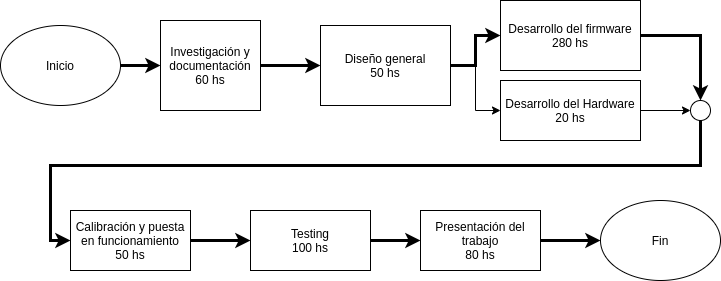
\includegraphics[width=1\textwidth]{./Figuras/AoN.png}
\caption{Diagrama en \textit{Activity on Node}}
\label{fig:AoN}
\end{figure}

\section{8. Diagrama de Gantt}
\label{sec:gantt}

\begin{figure}[htpb]
\centering 
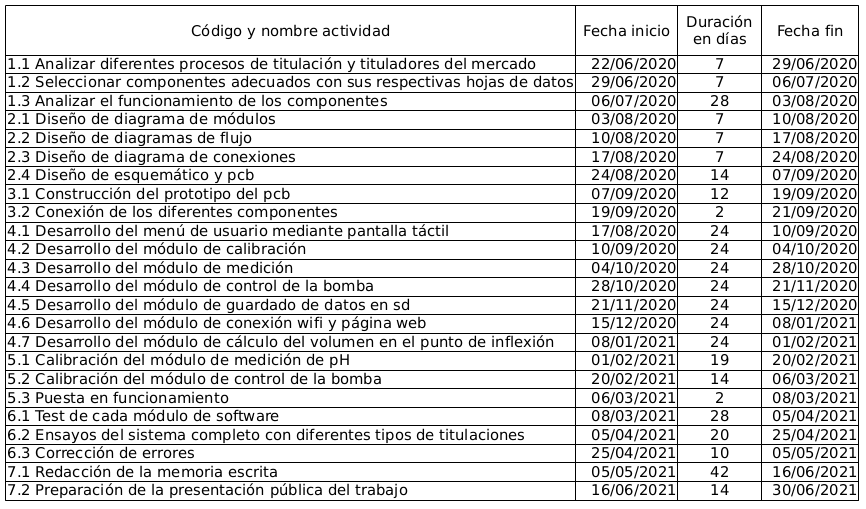
\includegraphics[width=1\textwidth]{./Figuras/TablaGantt.png}
\caption{Diagrama de Gantt: Tabla}
\label{fig:tablaGantt}
\end{figure}

\begin{figure}[htpb]

\centering 
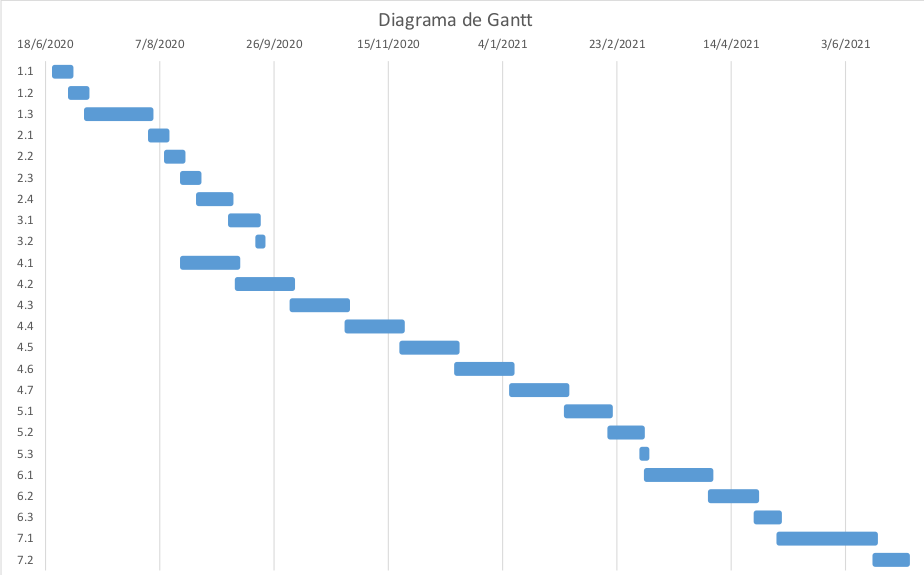
\includegraphics[width=1\textwidth]{./Figuras/DiagramaGantt.png}
\caption{Diagrama de Gantt: Gráfico}
\label{fig:diagramaGantt}
\end{figure}

\section{9. Matriz de uso de recursos de materiales}
\label{sec:recursos}

\begin{table}[htpb]
\label{tab:recursos}

\begin{tabularx}{\linewidth}{@{}|c|c|c|c|c|c|c|X|@{}}
\hline
\cellcolor[HTML]{C0C0C0} & \cellcolor[HTML]{C0C0C0} & \multicolumn{6}{c|}{\cellcolor[HTML]{C0C0C0}Recursos requeridos (horas)} \\ \cline{3-8} 
\multirow{-2}{*}{\cellcolor[HTML]{C0C0C0}\begin{tabular}[c]{@{}c@{}}Código\end{tabular}} & \multirow{-2}{*}{\cellcolor[HTML]{C0C0C0}\begin{tabular}[c]{@{}c@{}}Nombre\end{tabular}} 
& PC & Módulo  & Electrodo  & Bomba    & SD   & Insumos\\
\multirow{-2}{*}{\cellcolor[HTML]{C0C0C0}\begin{tabular}[c]{@{}c@{}} WBS\end{tabular}} & \multirow{-2}{*}{\cellcolor[HTML]{C0C0C0}\begin{tabular}[c]{@{}c@{}}  tarea\end{tabular}} &  & pantalla  &  &     &  & varios\\ \hline
1& Investigación  &60  &  &  &&  &\\
& documentación   &60  &  &  &&  &\\ \hline
2& Diseño general  &50  &  &  &&  &\\ \hline
3& Desarrollo de hardware &  &  &  & & &20\\ \hline
4& Desarrollo del firmware   &280  &  &  & & &\\ \hline
5& Calibración y puesta &5  &60  &30  &25 &5 &\\ 
5& en funcionamiento  &5  &60  &30  &25 &5 &\\ \hline
6& Testing 	 &100  &100  &100  &100 &100 &\\ \hline
7&Presentación del trabajo   &80  &  &  & & &\\ \hline
\end{tabularx}%
\end{table}


\section{10. Presupuesto detallado del proyecto}
\label{sec:presupuesto}


\begin{table}[htpb]
\centering
\begin{tabularx}{\linewidth}{@{}|X|c|r|r|@{}}
\hline
\rowcolor[HTML]{C0C0C0} 
\multicolumn{4}{|c|}{\cellcolor[HTML]{C0C0C0}COSTOS DIRECTOS} \\ \hline
\rowcolor[HTML]{C0C0C0} 
Descripción &
  \multicolumn{1}{c|}{\cellcolor[HTML]{C0C0C0}Cantidad} &
  \multicolumn{1}{c|}{\cellcolor[HTML]{C0C0C0}Valor unitario} &
  \multicolumn{1}{c|}{\cellcolor[HTML]{C0C0C0}Valor total} \\ \hline
 ESP32&
  \multicolumn{1}{c|}{1} &
  \multicolumn{1}{c|}{\$1400} &
  \multicolumn{1}{c|}{\$1400} \\ \hline
 Display táctil con lector SD&
  \multicolumn{1}{c|}{1} &
  \multicolumn{1}{c|}{\$1300} &
  \multicolumn{1}{c|}{\$1300} \\ \hline
Driver drv8825&
  \multicolumn{1}{c|}{2} &
  \multicolumn{1}{c|}{\$400} &
  \multicolumn{1}{c|}{\$800} \\ \hline
Modulo Ph-4502c&
  \multicolumn{1}{c|}{1} &
  \multicolumn{1}{c|}{\$4000} &
  \multicolumn{1}{c|}{\$4000} \\ \hline
Modulo Ph-4502c&
  \multicolumn{1}{c|}{1} &
  \multicolumn{1}{c|}{\$4000} &
  \multicolumn{1}{c|}{\$4000} \\ \hline
PCB&
  \multicolumn{1}{c|}{1} &
  \multicolumn{1}{c|}{\$500} &
  \multicolumn{1}{c|}{\$500} \\ \hline
\multicolumn{3}{|c|}{SUBTOTAL} &
  \multicolumn{1}{c|}{\$12000} \\ \hline
\rowcolor[HTML]{C0C0C0} 
\multicolumn{4}{|c|}{\cellcolor[HTML]{C0C0C0}COSTOS INDIRECTOS} \\ \hline
\rowcolor[HTML]{C0C0C0} 
Descripción &
  \multicolumn{1}{c|}{\cellcolor[HTML]{C0C0C0}Cantidad} &
  \multicolumn{1}{c|}{\cellcolor[HTML]{C0C0C0}Valor unitario} &
  \multicolumn{1}{c|}{\cellcolor[HTML]{C0C0C0}Valor total} \\ \hline
Insumos varios&
  \multicolumn{1}{c|}{1} &
  \multicolumn{1}{c|}{\$3000} &
  \multicolumn{1}{c|}{\$3000} \\ \hline

\multicolumn{3}{|c|}{SUBTOTAL} &
  \multicolumn{1}{c|}{3000} \\ \hline
\rowcolor[HTML]{C0C0C0}
\multicolumn{3}{|c|}{TOTAL} &\$15000
   \\ \hline
\end{tabularx}%
\end{table}


\section{11. Matriz de asignación de responsabilidades}
\label{sec:responsabilidades}

\begin{table}[htpb]

\centering
\resizebox{\textwidth}{!}{%
\begin{tabularx}{\linewidth}{@{}|X|c|X|X|X|X|@{}}
\hline
\rowcolor[HTML]{C0C0C0} 
\cellcolor[HTML]{C0C0C0} &
  \cellcolor[HTML]{C0C0C0} &
  \multicolumn{4}{c|}{\cellcolor[HTML]{C0C0C0}Listar todos los nombres y roles del proyecto} \\ \cline{3-6} 
\rowcolor[HTML]{C0C0C0} 
\cellcolor[HTML]{C0C0C0} &
  \cellcolor[HTML]{C0C0C0} &
  Responsable &
  Director &
  Colaboradores &
  Cliente \\ \cline{3-6} 
\rowcolor[HTML]{C0C0C0} 
\multirow{-3}{*}{\cellcolor[HTML]{C0C0C0}\begin{tabular}[c]{@{}c@{}}Código\\ WBS\end{tabular}} &
  \multirow{-3}{*}{\cellcolor[HTML]{C0C0C0}Nombre de la tarea} &
  \authorname &
  \supname &
  Anchino y Depetris &
  \clientename \\ \hline
1& Investigación  &P  &C & &C  \\ 
& documentación   & && &  \\ \hline
2& Diseño   &P  &I &C &A  \\ 
&  general  &  && & \\ \hline
3& Desarrollo  &P  &  &C  & \\ 
& de hardware &  &  &  & \\ \hline
4& Desarrollo   &P  &I &C &  \\ 
& del firmware   &  & & &  \\ \hline
5& Calibración  &P  &I &S &I  \\ \hline
6& Testing 	 &P  & & &I  \\ \hline
7&Presentación  &P  &A & &  \\ 
&del trabajo   & && &  \\ \hline
\end{tabularx}%
}
\end{table}

{\footnotesize
Referencias:
\begin{itemize}
	\item P = Responsabilidad Primaria
	\item S = Responsabilidad Secundaria
	\item A = Aprobación
	\item I = Informado
	\item C = Consultado
\end{itemize}
} %footnotesize


\section{12. Gestión de riesgos}
\label{sec:riesgos}

a) Identificación de los riesgos y estimación de sus consecuencias:
 
Riesgo 1 La presicición y resolución de las mediciones no cumplen con los requerimentos
\begin{itemize}
\item Severidad (S): 9 (nueve) porque la medición de volumen y de potencial son críticas para el resultado final.
\item Ocurrencia (O): 6 (seis) porque la medición del potencial puede verse afectada por el ruido, lo cual es bajo. La medición de volumen, en cambio, no se hace de manera directa ya que el prototipo inicial es un lazo abierto y depende exclusivamente de la presición de la bomba.
(ver que lo de lazo abierto este explicado antes y que este como requisito futuro un lazo cerrado)
\end{itemize} 

Riesgo 2 Caracteristicas del hardware seleccionado insuficientes para satisfacer las necesidades del sistema.
\begin{itemize}
\item Severidad (S): 8 (ocho) porque puede ocasionar funcionamiento defectuoso.
\item Ocurrencia (O): 2 (dos) porque se selecionó un procesador que puede hacer frente a los requerimientos establecidos, tanto presentes como futuros.
\end{itemize} 

Riesgo 3 Errores de diseño o fabricación en el prototipo del PCB
\begin{itemize}
\item Severidad (S): 7 (siete) porque puede ocasionar retrasos o daños en otros componentes.
\item Ocurrencia (O): 2 (dos) porque su diseño y fabricación serán verificados y validados por los colaboradores.
\end{itemize} 

Riesgo 4 Imposibilidad de cumplir los plazos planteados
\begin{itemize}
\item Severidad (S): 3 (tres) porque el cierre del proyecto del cual forma parte el SETPA es seis meses luego del plazo planteado como entrega del prototipo.
\item Ocurrencia (O): 5 (cinco) porque el contexto actual de aislamiento puede ocasionar demoras no previstas en la planificación.
\end{itemize} 

Riesgo 5: Imposibilidad de disponer del electrodo de pH
\begin{itemize}
\item Severidad (S): 10 (diez) porque es uno de los componentes fundamentales para el funciomiento del sistema.
\item Ocurrencia (O): 6 (seis) porque es un elemento que será suministrado por el grupo GISAI, en la medida que el financiamiento lo permita.
\end{itemize}


b) Tabla de gestión de riesgos:      (El RPN se calcula como RPN=SxO)

\begin{table}[htpb]
\centering
\begin{tabularx}{\linewidth}{@{}|X|X|X|X|X|X|X|@{}}
\hline
\rowcolor[HTML]{C0C0C0} 
Riesgo & S  & O  & RPN & S* & O* & RPN* \\ \hline
1      & 9  & 6  & 54  & 6  & 3  & 18     \\ \hline
2      & 8  & 2  & 16  &    &    &      \\ \hline
3      & 7  & 2  & 14  &    &    &      \\ \hline
4      & 3  & 5  & 15  &    &    &      \\ \hline
5      & 10 & 6  & 60  & 4  & 1  & 4      \\ \hline
\end{tabularx}%
\end{table}

Criterio adoptado: 
Se tomarán medidas de mitigación en los riesgos cuyos números de RPN sean mayores a 20

Nota: los valores marcados con (*) en la tabla corresponden luego de haber aplicado la mitigación.

c) Plan de mitigación de los riesgos que originalmente excedían el RPN máximo establecido:
 
Riesgo 1 Se realizarán pruebas en la presición y resolución de la bomba para evaluar si es necesario un lazo cerrado.
\begin{itemize}
\item Severidad (S): 6 (nueve) mediante la técnica de microstepping se puede ajustar la resolución de la bomba. La incorporación de un control de lazo cerrado se dejan tanto como requisito futuro de hardware y de software.
\item Ocurrencia (O): 3 (cuatro) porque se podrán realizar modificaciones a pedido en la bomba en caso de no cumplir con los requisitos de presición.
\end{itemize} 

Riesgo 5: Se utilizará un electrodo que dispone el laboratorio de química.
\begin{itemize}
\item Severidad (S): 4 (cuatro) porque permitirá realizar todas las pruebas y validaciones necesarias.
\item Ocurrencia (O): 1 (uno) porque se estableció como posibilidad en caso de no contar con el electrodo solicitado en tiempo y forma.
\end{itemize}



\section{13. Gestión de la calidad}
\label{sec:calidad}

\begin{enumerate}
\item Interfaces Externas
	\begin{enumerate}
	\item El hardware deberá contar con una pantalla TFT táctil. [TPA-ERH-01-REQ001]
	\begin{itemize}
\item Verificación: Se analizarán distintos módulos con sus respectivas hojas de datos.\\
\item Validación: El prototipo final debe funcionar con la pantalla TFT táctil seleccionada.\\
\end{itemize}
	\item El hardware deberá contar con un lector de tarjetas SD. [TPA-ERH-01-REQ002]
	\begin{itemize}
\item Verificación: Se analizarán distintos módulos con sus respectivas hojas de datos.\\
\item Validación: El prototipo final deberá guardar los datos de una titulación en una memoria SD\\
\end{itemize}
	\item El hardware deberá contar con un driver para un motor paso a paso Nema 17. [TPA-ERH-01-REQ003]
	\begin{itemize}
\item Verificación: Se analizarán distintos módulos con sus respectivas hojas de datos.\\
\item Validación: El motor de la bomba deberá girar la cantidad de pasos que el software envía.\\
\end{itemize}
	\item El hardware deberá contar con una entrada para un electrodo de pH. [TPA-ERH-01-REQ004]
	\begin{itemize}
\item Verificación: Se analizarán distintos módulos con sus respectivas hojas de datos.\\
\item Validación: El prototipo deberá funcionar con un electrodo conectado.\\
\end{itemize}
\end{enumerate}
	
\item Funciones
	\begin{enumerate}
	\item El usuario podrá elegir mediante la pantalla táctil los valores de tres muestras patrones (buffers) que se utilizarán en la calibración. [TPA-ERS-01-REQ001]
	\begin{itemize}
\item Verificación: Se implementará un menu de navegación que permita esta configuración.\\
\item Validación: Se realizará un prueba de calibración.\\
\end{itemize}
El usuario podrá elegir mediante la pantalla táctil el volumen de corte de la titulación. [TPA-ERS-01-REQ002]
\begin{itemize}
\item Verificación: Se implementará un menu de navegación que permita esta configuración.\\
\item Validación: Se realizará una titulación y se verificará si la cantidad de volumen inyectado se corresponde con el volumen de corte.\\
\end{itemize}
	\item El usuario podrá elegir mediante la pantalla táctil si utilizar o no el agitador. Cuando el proceso de titulación comience, el agitador debe activarse si así lo indicó el usuario. [TPA-ERS-01-REQ003]
	\begin{itemize}
\item Verificación: Se implementará un menu de navegación que permita esta configuración.\\
\item Validación: El motor del agitador encenderá si la opción esta activada\\
\end{itemize}
	\item El usuario podrá realizar mediante la pantalla táctil el proceso de calibración con cada uno de los tres buffers. [TPA-ERS-01-REQ004]
	\begin{itemize}
\item Verificación: Se implementará un menu de navegación que permita la calibración.\\
\item Validación: Se realizará una medición y se constatará con un instrumento patrón.\\
\end{itemize}
	\item Los valores de potencial obtenidos en el proceso de la calibración se deben guardar en la memoria flash del ESP32. [TPA-ERS-01-REQ005]
	\begin{itemize}
\item Verificación: Se implementará una función que realice el guardado en memoria.\\
\item Validación: Se leerá los datos guardados luego de realizar un corte de energía al sistema.\\
\end{itemize}
	\item El valor de pH se debe calcular de manera proporcional a la recta de ajuste de los valores de potencial obtenidos en la calibración. [TPA-ERS-01-REQ006]
	\begin{itemize}
\item Verificación: Se implementará una función que calcule la recta de ajuste.\\
\item Validación: Se realizará una medición y se constatará con un instrumento patrón.\\
\end{itemize}
	\item El usuario podrá dar inicio al proceso de titulación mediante la pantalla táctil. [TPA-ERS-01-REQ007]
	\begin{itemize}
\item Verificación: Se implementará una opción que permita dar inicio al proceso.\\
\item Validación: Se hará una prueba de titulación.\\
\end{itemize}
	\item Durante la titulación, la pantalla debe mostrar el valor actual leído en mV y en pH y una gráfica de pH en el eje de la ordenadas y de volumen de titulante añadido en el eje de las abcisas. [TPA-ERS-01-REQ008]
	\begin{itemize}
\item Verificación: Se implementará una función que calcule y muestre los valores solicitados.\\
\item Validación: Se hará una prueba de titulación.\\
\end{itemize}

	\item Cada valor de volumen añadido junto al valor de potencial asociado durante el proceso de titulación deben almacenarse en un archivo de texto en la tarjeta sd. No es necesario que esto se haga en tiempo real. Al iniciar otro proceso de titulación, los datos de la titulación anterior serán eliminados. [TPA-ERS-01-REQ009]
	\begin{itemize}
\item Verificación: Se implementará una función que realice el guardado en memoria.\\
\item Validación: Se leeran los datos guardados de una titulación a través de una computadora.\\
\end{itemize}

	\item Cada valor de volumen añadido junto al valor de potencial asociado durante el proceso de titulación deben mostrarse en una página web almacenada en la memoria flash. [TPA-ERS-01-REQ010]
	\begin{itemize}
\item Verificación: Se implementará una función que escriba los datos en una pagina web almacenada en memoria.\\
\item Validación: Se leerá la página web luego de realizar una titulación.\\
\end{itemize}

	\item El usuario podrá acceder a la página web mediante una conexión wifi. No es necesario que esto se haga en tiempo real. [TPA-ERS-01-REQ011]
	\begin{itemize}
\item Verificación: Se mostrarán en pantalla los datos de conexión para que un usuario pueda acceder a la red mediante un dispositivo externo.\\
\item Validación: Se conectará una dispositivo a la red generada por el módulo wifi para acceder a la página web.\\
\end{itemize}

	\item El sistema deberá ser capaz de leer y mostrar el potencial entregado por un electrodo de pH, con una resolución de 1 mV para la lectura del potencial y de 0.01 pH para su conversión a pH. Para ello se utilizará el conversor analógico de 12 bits incorporado en el ESP32. [TPA-ERS-01-REQ012]
	\begin{itemize}
\item Verificación: Se implementará una función que calcule el valor de pH y de potencial a través de la medición del ADC.\\
\item Validación: Se alimentará la entrada del ADC con una fuente de tensión regulable con una resolución mínima de 1 mV. Se variará la tensión de la fuente para abarcar el rango de 0 a 5 V.\\
\end{itemize}

	\item El sistema deberá enviar pulsos de 10 ms de ciclo útil al pin step del módulo dvr8825. El tiempo mínimo de espera entre cada pulso debe ser de 1 segundo luego que la lectura de potencial se haya estabilizado. El sistema dejará de enviar los pulsos cuando se haya inyectado la cantidad de volumen indicada por el usuario como volumen de corte. [TPA-ERS-01-REQ013]
	\begin{itemize}
\item Verificación: Se implementará una función que envie por un puerto digital la salida especificada.\\
\item Validación: Se conectará un osciloscopio al pin digital para medir la salida.\\
\end{itemize}

	\item Cada pulso se corresponde con el incremento de TBD mL en la cantidad de volumen inyectado, comenzando por un nivel de 0 mL. [TPA-ERS-01-REQ014]
		\begin{itemize}
\item Verificación: Se implementará una función que realice el cálculo del volumen.\\
\item Validación: Se realizará la medición en comparación con un instrumento patrón.\\
\end{itemize}


\end{enumerate}

\item Requisitos de Rendimiento
	\begin{enumerate}
	\item El sistema deberá ser capaz de realizar titulaciones que involucren una cantidad mínima de 50 ml 	\item de titulante y una cantidad máxima de 100 ml. [TPA-ERS-01-REQ016]
	\begin{itemize}
\item Verificación: Se establecerán los limite en las funciones correspodientes.\\
\item Validación: Se realizará una titulación de 50 ml y otra de 100 ml.\\
\end{itemize}
	\end{enumerate}
	
\item Restricciones de Diseño
	\begin{enumerate}
	\item Se utilizará el módulo ESP32 como computadora principal. [TPA-ERS-01-REQ017]
	\begin{itemize}
\item Verificación: Se analizarán las hojas de datos del módulo.\\
\item Validación: El prototipo deberá funcionar con el módulo ESP32.\\
\end{itemize}

	\end{enumerate}
	
\end{enumerate}

\section{14. Comunicación del proyecto}
\label{sec:comunicaciones}

El plan de comunicación del proyecto es el siguiente:

% Please add the following required packages to your document preamble:
% \usepackage{graphicx}
% \usepackage[table,xcdraw]{xcolor}
% If you use beamer only pass "xcolor=table" option, i.e. \documentclass[xcolor=table]{beamer}
\begin{table}[htpb]
%\centering
\resizebox{\textwidth}{!}{%
\begin{tabularx}{\linewidth}{@{}|X|X|X|X|X|X|@{}}
\hline
\rowcolor[HTML]{C0C0C0} 
\multicolumn{6}{|c|}{\cellcolor[HTML]{C0C0C0}PLAN DE COMUNICACIÓN DEL PROYECTO}           \\ \hline
\rowcolor[HTML]{C0C0C0} 
¿Qué comunicar? & Audiencia & Propósito & Frecuencia & Método de comunicac. & Responsable \\ \hline
Plan del proyecto & Director, cliente y colaboradores & Informar sobre inicio del proyecto & Una vez & Reunión virtual & Fernando Daniele       \\ \hline
Grado de avance & Director  & Informar y validar & Mensual & Correo electrónico & Fernando Daniele \\ \hline
Consultas       & Colaboradores & Informar, buscar soluciones & Cuando sea necesario & Correo electrónico                      & Fernando Daniele \\ \hline
Problemas que pongan en peligro la ejecución del proyecto & Director & Brindar soporte y sugerencias & Cuando sea necesario &  Reunión virtual o correo electrónico & Fernando Daniele \\ \hline
Finalización y cierre  & Director y jurados  & Informar, evaluar & Una vez & Correo electrónico & Fernando Daniele \\ \hline
\end{tabularx}%
}
\end{table}

\section{15. Gestión de Compras}
\label{sec:compras}

Las compras necesarias para la fabricación del prototipo serán ejecutadas por el grupo GISAI bajo los proveedores y protocolos sugeridos por la UTN FRSFCO.


\vspace{55px}


\section{16. Seguimiento y control}
\label{sec:seguimiento}

\begin{table}[!htpb]
\centering
\begin{tabularx}{\linewidth}{@{}|X|X|X|X|X|X|@{}}
\hline
\rowcolor[HTML]{C0C0C0} 
\multicolumn{6}{|c|}{\cellcolor[HTML]{C0C0C0}SEGUIMIENTO DE AVANCE}                                                                       \\ \hline
\rowcolor[HTML]{C0C0C0} 
Tarea del WBS & Indicador de avance & Frecuencia de reporte & Resp. de seguimiento & Persona a ser informada & Método de comunic. \\ \hline
1 & Cantidad de componentes investigados y documentados & Mensual & Fernando Daniele  & Director & Correo electrónico  \\ \hline
2 & Cantidad de diagramas diseñados & Mensual & Fernando Daniele  & Director & Correo electrónico  \\ \hline
3 & Cantidad de componentes soldados / conectados  & Mensual & Fernando Daniele  & Director & Correo electrónico  \\ \hline 
4 & Cantidad de funciones implementadas &  Mensual & Fernando Daniele  & Director & Correo electrónico  \\ \hline
5 & Cantidad de módulos calibrados & Mensual & Fernando Daniele & Director & Correo electrónico  \\ \hline
6 & Cantidad de ensayos y correcciones realizadas & Mensual & Fernando Daniele  & Director & Correo electrónico  \\ \hline
7 & Cantidad de secciones escritas & Mensual & Fernando Daniele  & Director & Correo electrónico  \\ \hline
\end{tabularx}%
%}
\end{table}

\section{17. Procesos de cierre}    
\label{sec:cierre}

Al finalizar el proyecto, el responsable realizará una reunión final de evaluación que contemplará las siguientes actividades:

\begin{itemize}
\item Se compararán los tiempos reales de ejecución con los planificados.
\item Se verificará si los requisitos solicitados por el cliente fueron totalmente cumplidos.
\item Se identificará las técnicas y procedimientos útiles e inútiles que se utilizaron para cumplir cada una de las actividades propuestas.
\item Se identificará cada problema o incoveniente que haya ocasionado un desvío en la ejecución normal del proyecto con sus repectivas soluciones.
\item Se dará agradecimiento a todos los interesados, y en especial al equipo de trabajo y colaboradores.
\end{itemize}

\end{document}
